\documentclass[chi_draft]{sigchi}

% Use this command to override the default ACM copyright statement
% (e.g. for preprints).  Consult the conference website for the
% camera-ready copyright statement.

%% EXAMPLE BEGIN -- HOW TO OVERRIDE THE DEFAULT COPYRIGHT STRIP -- (July 22, 2013 - Paul Baumann)
% \toappear{Permission to make digital or hard copies of all or part of this work for personal or classroom use is      granted without fee provided that copies are not made or distributed for profit or commercial advantage and that copies bear this notice and the full citation on the first page. Copyrights for components of this work owned by others than ACM must be honored. Abstracting with credit is permitted. To copy otherwise, or republish, to post on servers or to redistribute to lists, requires prior specific permission and/or a fee. Request permissions from permissions@acm.org. \\
% {\emph{CHI'14}}, April 26--May 1, 2014, Toronto, Canada. \\
% Copyright \copyright~2014 ACM ISBN/14/04...\$15.00. \\
% DOI string from ACM form confirmation}
%% EXAMPLE END -- HOW TO OVERRIDE THE DEFAULT COPYRIGHT STRIP -- (July 22, 2013 - Paul Baumann)

% Arabic page numbers for submission.  Remove this line to eliminate
% page numbers for the camera ready copy
\pagenumbering{arabic}

% Load basic packages
\usepackage{balance}  % to better equalize the last page
%\usepackage{graphics} % for EPS, load graphicx instead 
\usepackage{graphicx}
\usepackage{caption}
\usepackage{subcaption}
\usepackage[T1]{fontenc}
\usepackage{txfonts}
\usepackage{mathptmx}
\usepackage[pdftex]{hyperref}
\usepackage{color}
\usepackage{booktabs}
\usepackage{textcomp}
% Some optional stuff you might like/need.
\usepackage{microtype} % Improved Tracking and Kerning
% \usepackage[all]{hypcap}  % Fixes bug in hyperref caption linking
\usepackage{ccicons}  % Cite your images correctly!
\usepackage[utf8]{inputenc} % for a UTF8 editor only
\usepackage{tikz}
\newcommand*\circled[1]{\tikz[baseline=(char.base)]{
            \node[shape=circle,draw,inner sep=2pt] (char) {#1};}} % circled icons for images
						
% If you want to use todo notes, marginpars etc. during creation of your draft document, you
% have to enable the "chi_draft" option for the document class. To do this, change the very first
% line to: "\documentclass[chi_draft]{sigchi}". You can then place todo notes by using the "\todo{...}"
% command. Make sure to disable the draft option again before submitting your final document.
\usepackage{todonotes}

% Paper metadata (use plain text, for PDF inclusion and later
% re-using, if desired).  Use \emtpyauthor when submitting for review
% so you remain anonymous.
\def\authorname{Tobias Lahmann}
\def\plaintitle{TITLE TITLE TITLE}
\def\plainauthor{\authorname}
\def\emptyauthor{}
\def\plainkeywords{Virtual Reality, psychology, research}
\def\plaingeneralterms{Documentation, Standardization}

% llt: Define a global style for URLs, rather that the default one
\makeatletter
\def\url@leostyle{%
  \@ifundefined{selectfont}{
    \def\UrlFont{\sf}
  }{
    \def\UrlFont{\small\bf\ttfamily}
  }}
\makeatother
\urlstyle{leo}

% To make various LaTeX processors do the right thing with page size.
\def\pprw{8.5in}
\def\pprh{11in}
\special{papersize=\pprw,\pprh}
\setlength{\paperwidth}{\pprw}
\setlength{\paperheight}{\pprh}
\setlength{\pdfpagewidth}{\pprw}
\setlength{\pdfpageheight}{\pprh}

% Make sure hyperref comes last of your loaded packages, to give it a
% fighting chance of not being over-written, since its job is to
% redefine many LaTeX commands.
\definecolor{linkColor}{RGB}{6,125,233}
\hypersetup{%
  pdftitle={\plaintitle},
  pdfauthor={\plainauthor},
%  pdfauthor={\emptyauthor},
  pdfkeywords={\plainkeywords},
  bookmarksnumbered,
  pdfstartview={FitH},
  colorlinks,
  citecolor=black,
  filecolor=black,
  linkcolor=black,
  urlcolor=linkColor,
  breaklinks=true,
}

% create a shortcut to typeset table headings
% \newcommand\tabhead[1]{\small\textbf{#1}}

% End of preamble. Here it comes the document.
\begin{document}

\title{\plaintitle}

\numberofauthors{1}
\author{
	\alignauthor{\authorname\\
		\affaddr{Research Trends in Media Informatics}\\
		\affaddr{Ulm, Germany}\\
		\email{tobias.lahmann@uni-ulm.de}}
}

\maketitle
%----------------------------------------------------------------------------------------
%	Document
%----------------------------------------------------------------------------------------

\begin{abstract}
Virtual Reality techniques are very well suited for games as they incorporate users into the action and offer great potential for developers to extend the experience conveyed in their games. Understanding the advantages but also the disadvantages of VR in all fields of gaming is important for the future advancement of the fields.
The many varying aspects and different field of needed research for \textit{Games in VR} will be examined here.
Other literature is often focusing either on the field of games and analyzing the game-impacts on players or the psychological affects of games, or is studying the field of virtual reality and the affects of this.
The objective of this publication is to combine both fields and show future development of games in virtual reality.
\end{abstract}


\category{H.5.1}{[Multimedia Information Systems]: Artificial, augmented, and virtual realities}{}{}

\keywords{\plainkeywords}


\section{Introduction}
%\todo[inline]{write introduction}

The virtual generation and perception of real environments or imaginary settings, rendered by a computer using specialized software, is referred to as virtual reality (VR). Its goal is to simulate a user's physical presence in this environment, by enabling the user to interact with this space and any objects depicted therein using specialized display screens or projectors and other devices.

The potential of virtual reality in gaming is an enormous factor both for the scientific and commercial regarding its multitude of use cases. 

In the past decade a variety of electronic devices has reached the marked and found its way into the homes of consumers. Gaming consoles have become entertainment systems offering more than just the gaming aspect. Computers gained the abilities of past supercomputers and are far more than workstations for the majority of modern population. With technological advancements made in the past 50 Years and popularity gains of these systems also the gaming industry has reached its heyday. 

VR, although expensive, gains more interest and the audience grows almost daily. 
Games that do not naturally support VR are searching for ways to include VR in their games, described in the section \textit{Games And VR}\ref{sec:gamesNvr}.

\begin{figure}%[h]
	\centering
	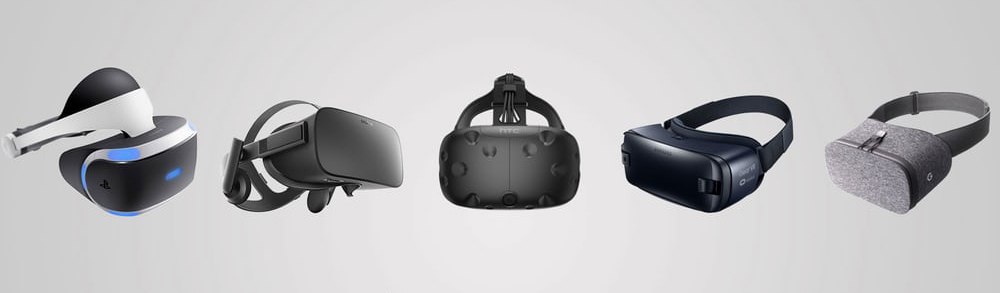
\includegraphics[width=0.99\columnwidth]{./figures/vr-hmd}
	\caption[vr-hmd]{Overview of different consumer HMD as available in late 2016. FLTR Plystation VR, Oculus Rift, HTC Vive, Samsung Gear VR, Daydream View.\footnotemark}~\label{fig:vrHMD}
\end{figure}
\footnotetext{\textcopyright~Newatlas, [Online; accessed January 04., 2017],[Digitally revised] \url{http://img-2.newatlas.com/vr-comparison-2016-b-2.jpg}}

The development of consumer friendly head mounted devices (HMD) for VR, as to see in \textbf{Figure~\ref{fig:vrHMD}}, has just picked up in recent years with systems like the \textit{Oculus Rift in March 2016}, the \textit{HTC Vive in April 2016}, the \textit{Samsung Gear VR in August 2015}, the \textit{Playstation VR in October 2015} or the \textit{Daydream View in November 2015}. 

Many developers have already started to develop games that use the advances of VR and are serving quick, but the research on this fields has lacked behind on reliable results regarding the ideal approach to points such as immersion, interaction and performance. This publication intends to show the many disciplines and what research can be done to improve VR in Games.



\section{Discussion}


\section{Summary}


\section{Conclusion}
\textbf{Virtual reality games can and will undergo a lot of changes, especially with the general development of VR in the near future. It will, however, take time, money, and a combined effort on the part of many people.}

VR and HMD are not yet core technologies in todays gaming society but I am being confident that this will change rapidly and the advantages will quickly adapt to many areas of our every day life, as well as gaming.

Almost all of the senses of the human body can be reached with todays technology. Some people may like the thought of totally immersed gaming, other find it disturbing.\newline
Although a controversy appears in some fields the research will surely go on in the next years bringing many innovative and tense devices to our lives including better interaction, conclusive visual effects, stunning audio and astonishing touchable illusions. 

There are just many ways of finding new ways to improve VR gaming in the future. VR is on the edge of becoming a main way to experience games and the enormous potential offers just too many aspects to consider in one paper.


% Referenzen
% References must be the same font size as other body text.
\bibliographystyle{SIGCHI-Reference-Format}
\bibliography{citation}


\end{document}

%%% Local Variables:
%%% mode: latex
%%% TeX-master: t
%%% End:
